\chapter{Resonance Compensation Studies at the CERN Proton Synchrotron Booster}
\label{sec:ch5}

\section{General Description}
The Proton Synchrotron Booster (PSB) is the first circular accelerator in the CERN accelerator complex that ultimately leads to the LHC. Figure \ref{fig:cernac} shows the entire chain of accelerators at CERN, feeding a variety of physics experiments \cite{cernplot}. Following the successful implementation of the LHC Injectors Upgrade (LIU) \cite{liu}, the PSB receives $H^-$ ion beam coming from the Linac4 at an energy of 160 MeV. Interestingly enough, the PSB is not just one ring, but rather four synchrotron rings stacked on top of each other. This is to counteract space charge effects which are largest at low energy machines. Once the ion beam enters the PSB rings, the electrons are stripped off with a carbon foil and proton beam is achieved \cite{psbstrip}. The proton beam is then accelerated from an energy of 160 MeV to 2 GeV. The beam from the four rings gets merged together and then gets injected to the Proton Synchrotron (PS). This is true for LHC-type beams, nevertheless, the PSB can also accelerate lead ions and deliver to other customers like the heavy ion experiments like ISOLDE \cite{foteini1}.   \cite{foteini2} 

\begin{figure}[H]
    \centering
    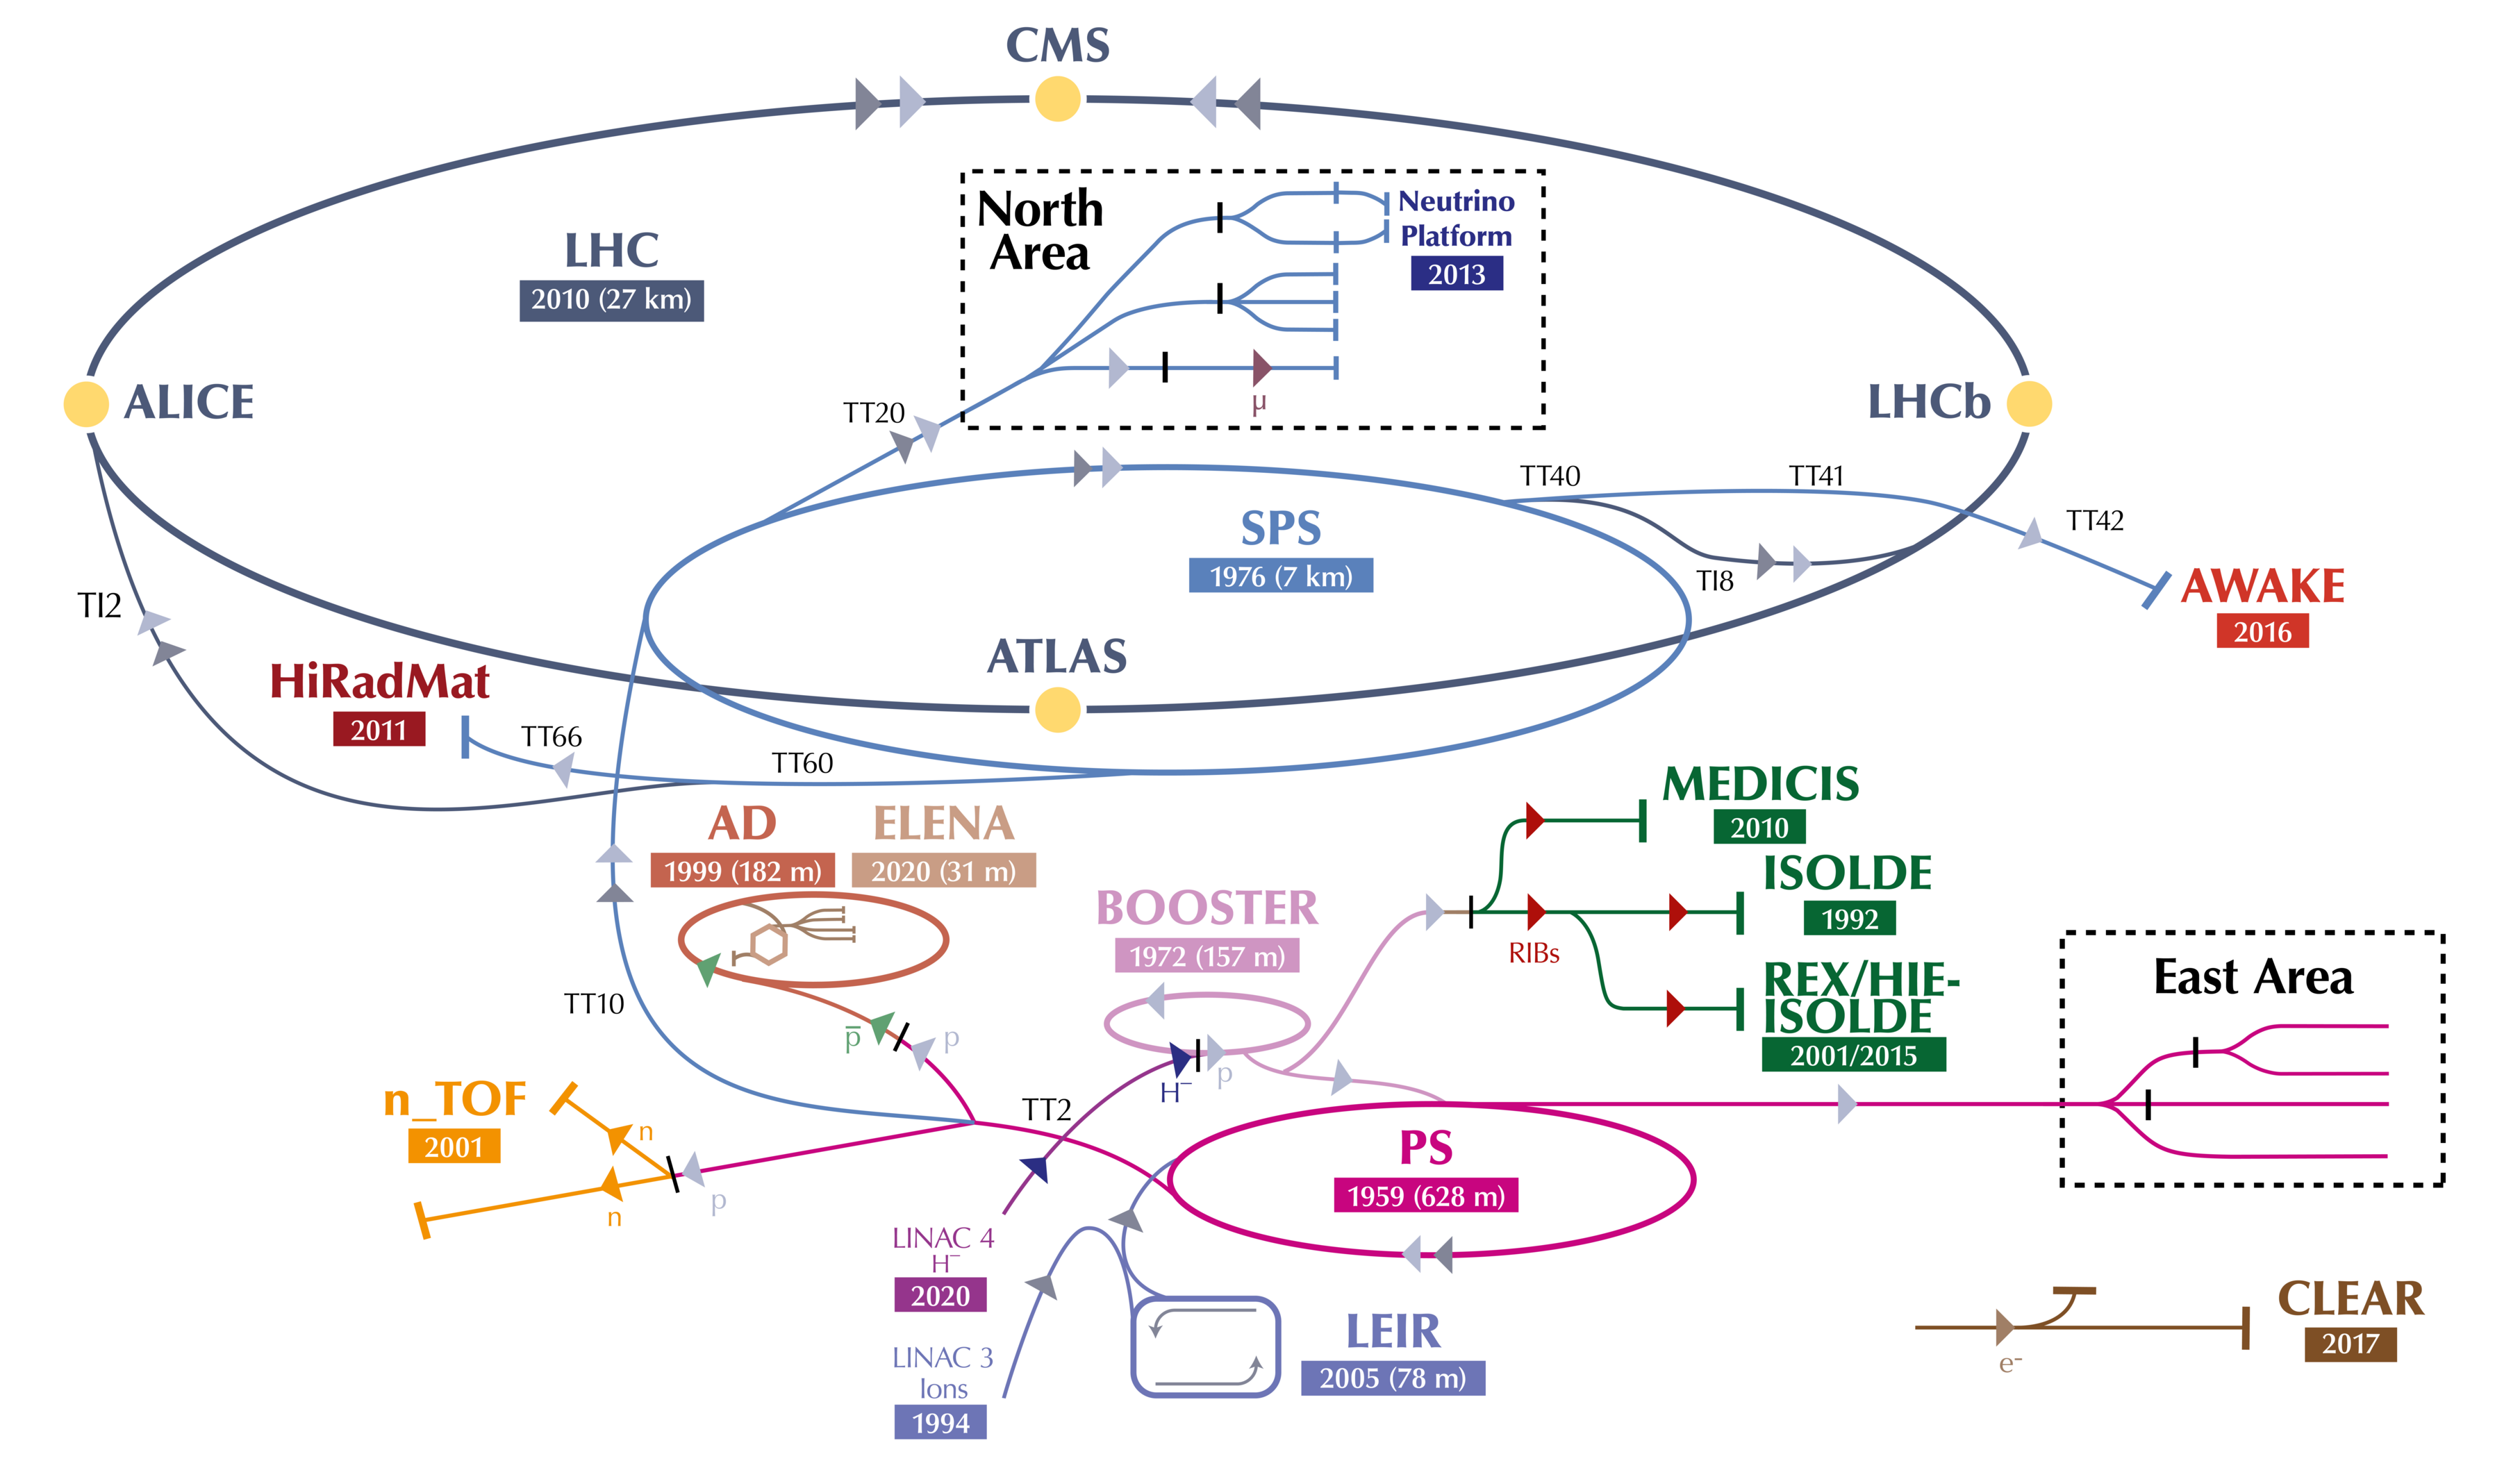
\includegraphics[width=\linewidth]{chapter5/CERN_AC.png}
    \caption{A graphic overview of all accelerators in operation at CERN as of 2022. Original image taken from Ref. \cite{cernplot}. This file is licensed under the Creative Commons Attribution 4.0 International license.}
    \label{fig:cernac}
\end{figure}

\section{Tune Diagram and Operation}

\begin{figure}[H]
    \centering
    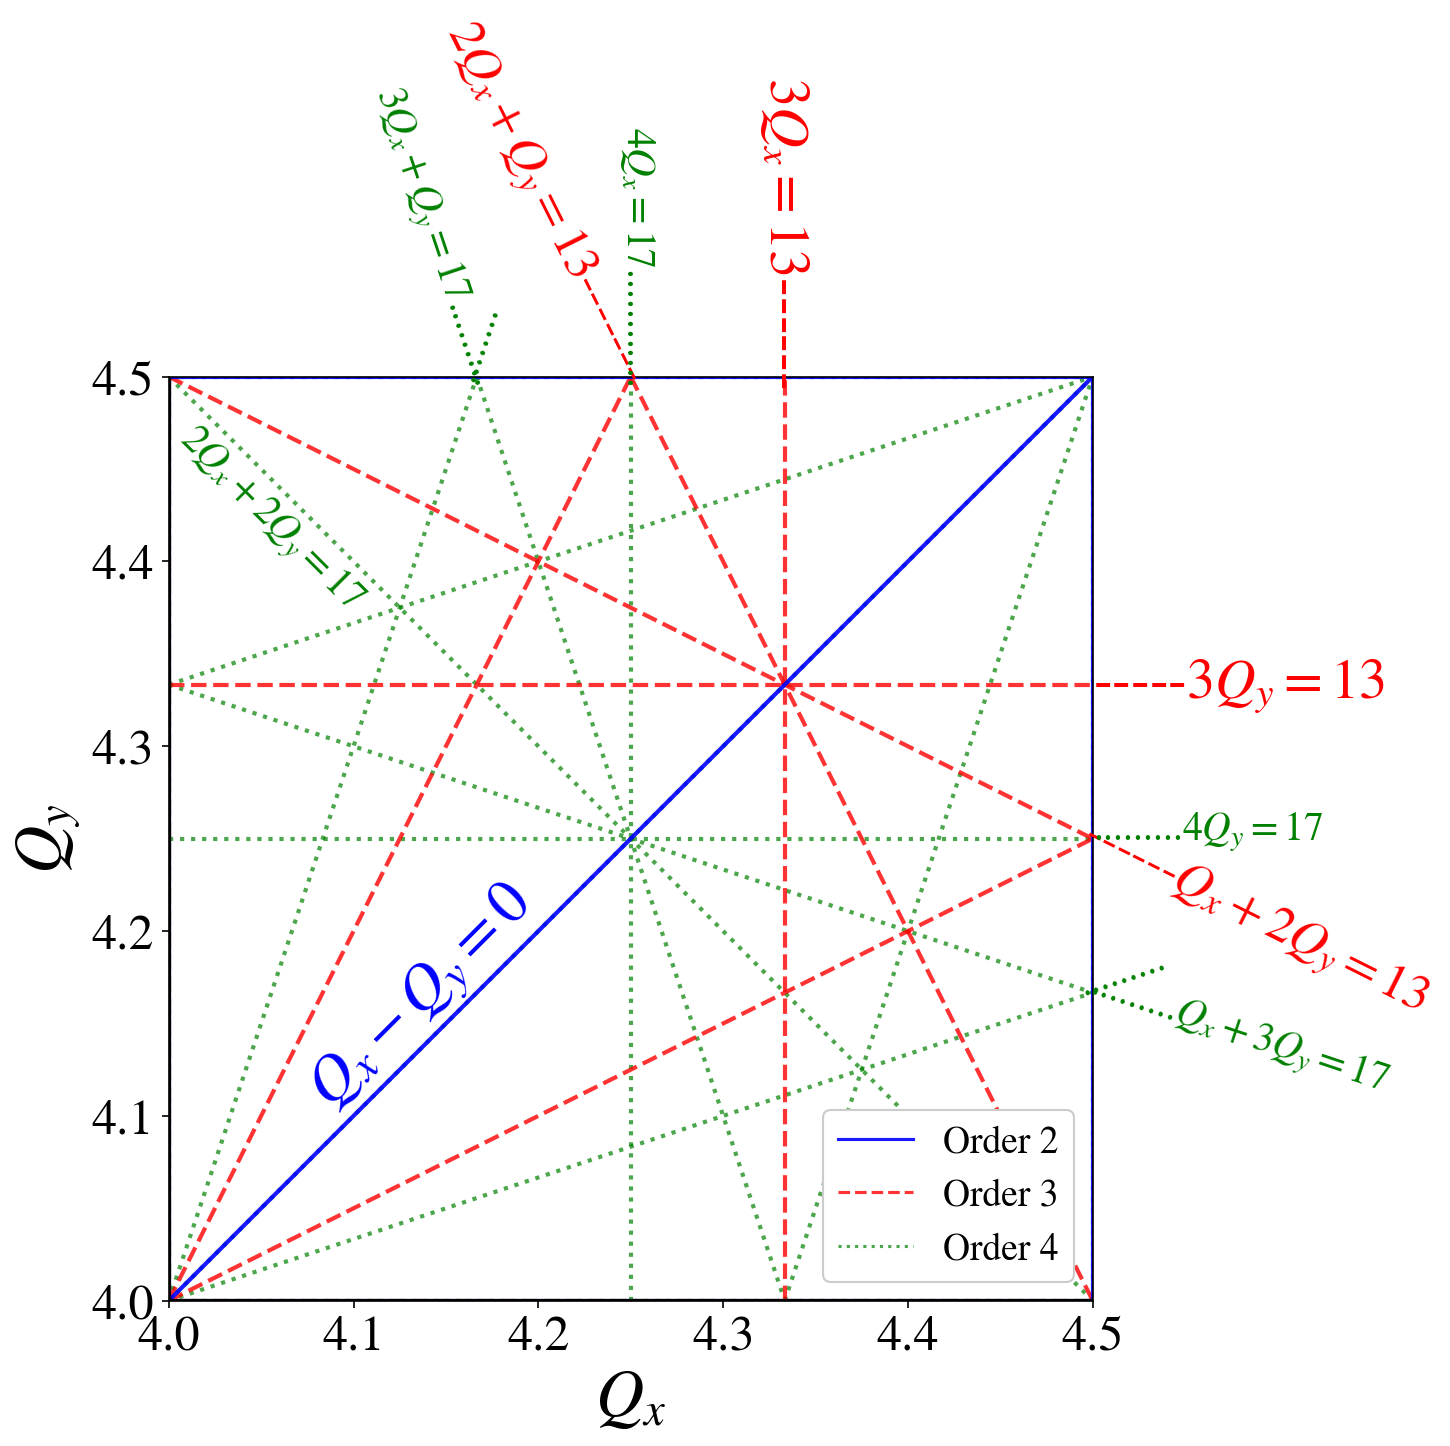
\includegraphics[width=\linewidth]{chapter5/psb_td.png}
    \caption{Portion of the tune diagram enclosing the operational tunes of the PS Booster with relevant resonance lines labelled}
    \label{fig:psbtd}
\end{figure}

\begin{figure}[H]
    \centering
    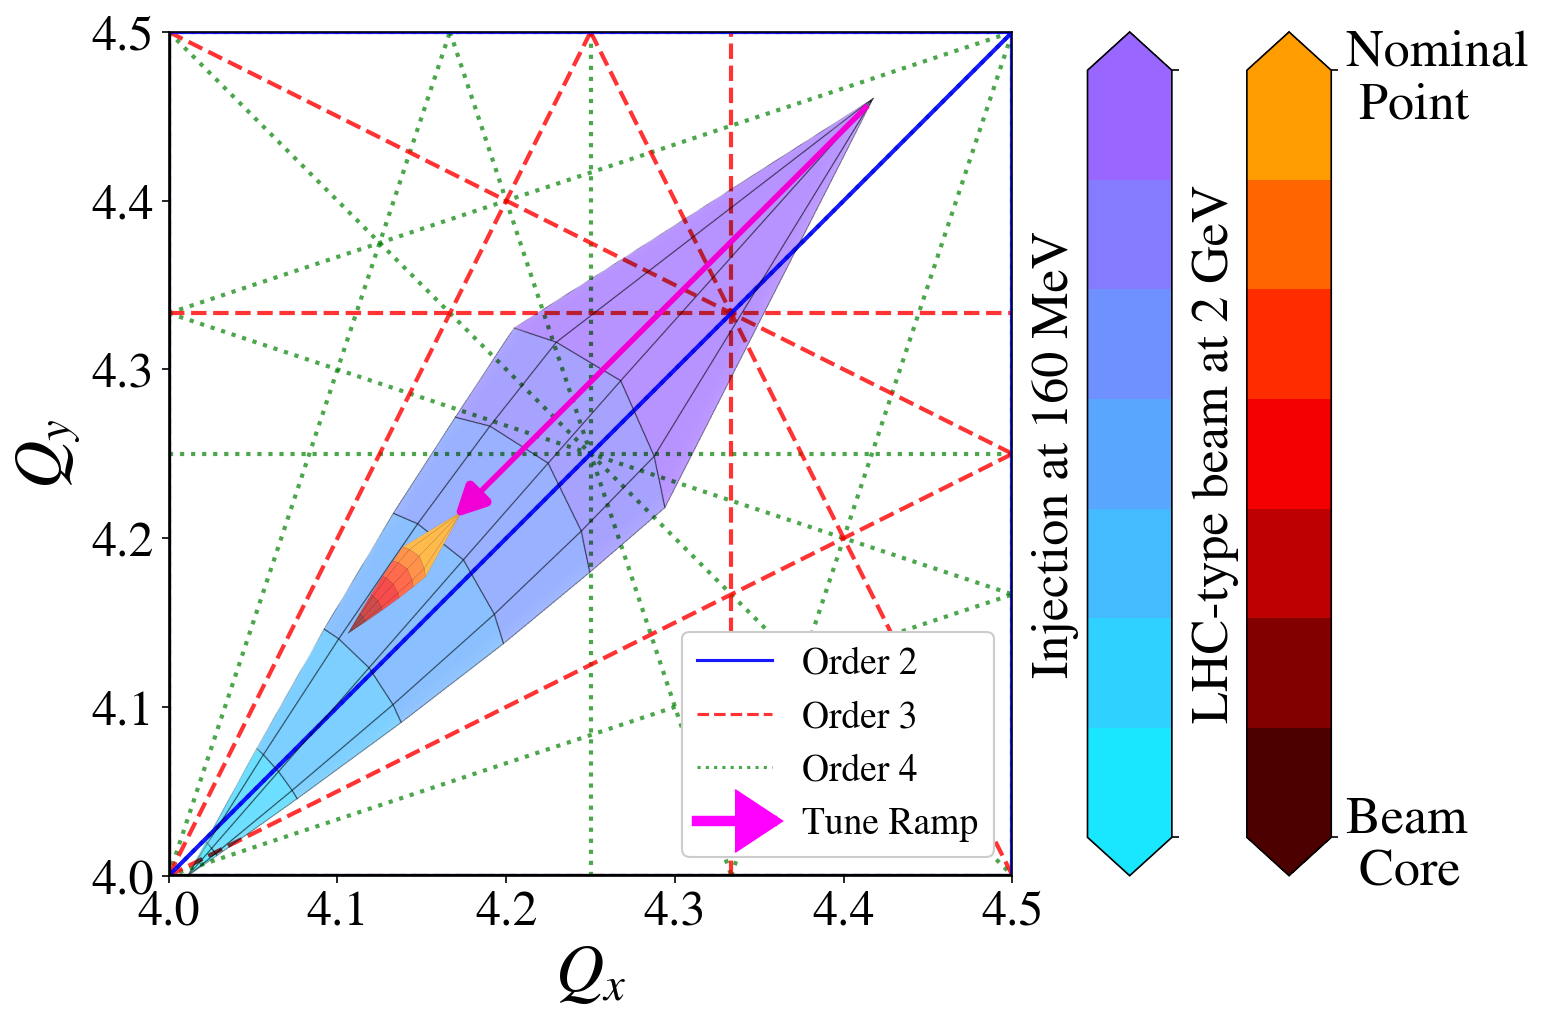
\includegraphics[width=\linewidth,keepaspectratio]{chapter5/operational.png}
    \caption{Operational tune footprint for PSB beam at injection (cool color map) and footprint after beam has been accelerated to 2 GeV (warm color map)}
    \label{fig:operational_psb}
\end{figure}

\section{Optimization Algorithms for Resonance Compensation}

\cite{geoff}

\begin{figure}[H]
    \centering
    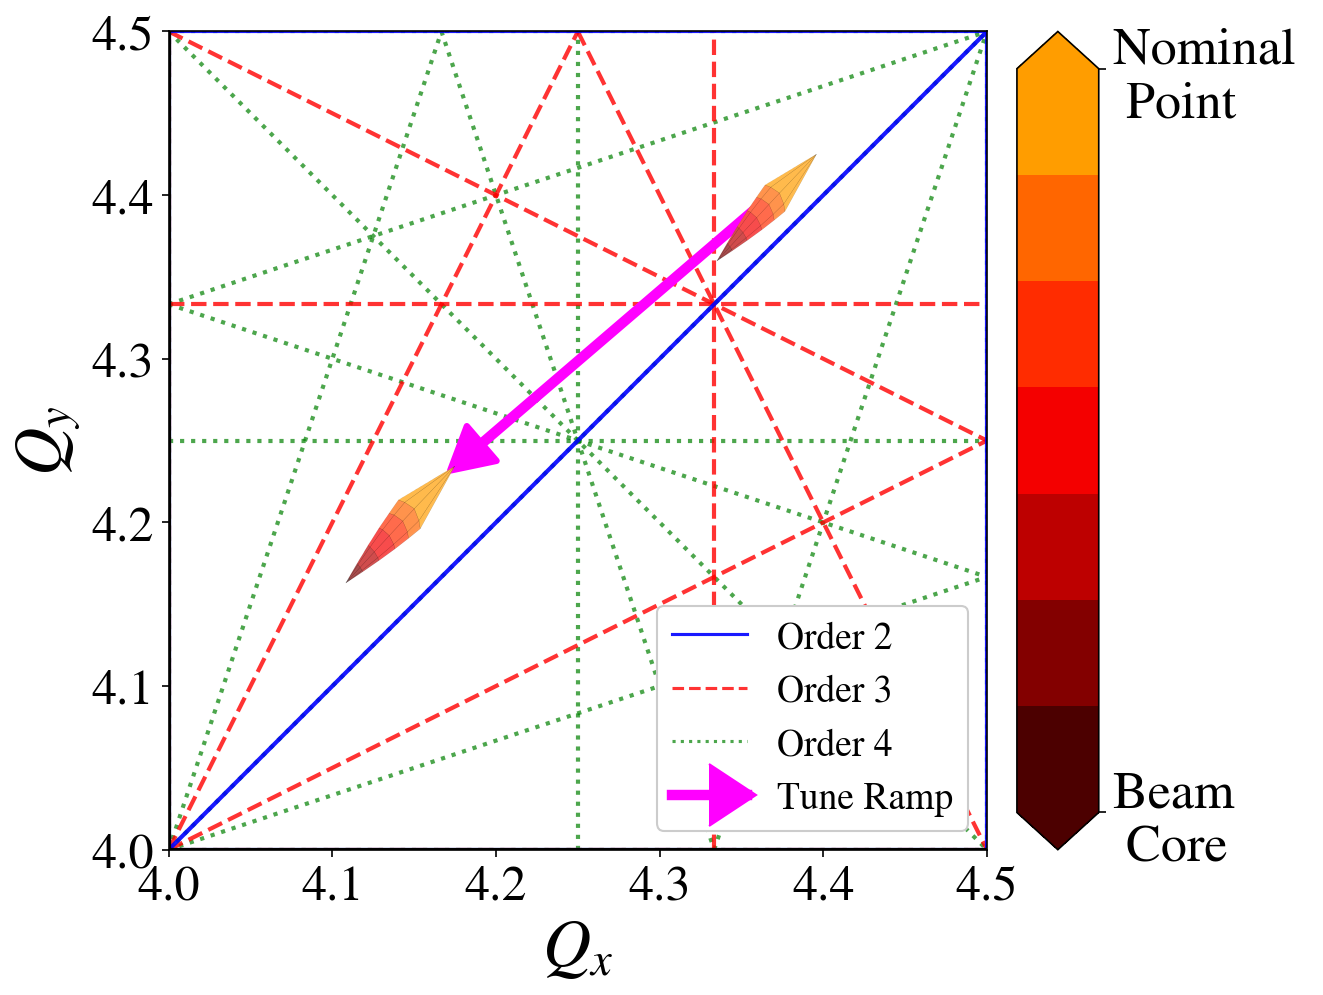
\includegraphics[width=\linewidth]{chapter5/experiment.png}
    \caption{Experimental setup of the tune diagram dynamics for the optimization of resonance compensation used in the PS Booster.}
    \label{fig:experimentPSB}
\end{figure}

\begin{table}[H]
    \centering
    \caption{List of elements in the PS Booster at CERN used for resonance compensation optimization as present in all four PS Booster rings.}
    \label{tab:psbcomp}
    \begin{tabular}{|c|c|}
    \hline
    \textbf{Name} & \textbf{Type}    \\ \hline
    XN04L1    & Normal Sextupole \\ \hline
    XN06L1    & Normal Sextupole \\ \hline
    XN09L1    & Normal Sextupole \\ \hline
    XN012L1    & Normal Sextupole \\ \hline
    XN0311L1    & Normal Sextupole   \\ \hline
    XN0816L1    & Normal Sextupole   \\ \hline
    ON0311L1    & Normal Octupole  \\ \hline
    ON0816L1    & Normal Octupole   \\ \hline
    XSK2L4    & Skew Sextupole  \\ \hline
    XSK4L1    & Skew Sextupole   \\ \hline
    XSK6L4    & Skew Sextupole   \\ \hline
    \end{tabular}
\end{table}

\subsection{Bayesian Optimization}

\subsection{BOBYQA (Bound Optimization BY Quadratic Approximation)}

\section{Experimental Verification of Compensation}
